\documentclass{article}
\usepackage[utf8]{inputenc}
\usepackage[T1]{fontenc}
\usepackage{graphicx}
\usepackage{hyperref}
\usepackage{geometry}
\geometry{margin=1in}

\title{HYDROSTATICS (Plate CCXXXIX)}
\date{Encyclopaedia Britannica (1771)}

\begin{document}
\maketitle

\section*{Historical source}
\textbf{Entry ID:} \texttt{entry-britannica-volume-149982181-row-270-270} \\
\textbf{Volume ID:} 149982181 \\
\textbf{Character Count:} 993

\subsection*{Extracted Text}
HYDROSTATICS. Plate CCXXXIX.

[HISTORICAL COPPERPLATE ENGRAVING: HYDROSTATICS (Plate CCXXXIX)]
Category: Physics and Fluid Mechanics
Visual Description: Detailed 18th-century copperplate engraving illustrating principles of hydrostatics and fluid equilibrium. Depicts experimental apparatus demonstrating hydrostatic pressure, communicating vessels, and the hydrostatic paradox (water level equilibrium regardless of vessel shape). Includes apparatus for measuring specific gravity, siphons, and buoyant force diagrams.
Identified Engraved Figures:
  * Fig. 1: Communicating vessels demonstrating uniform hydrostatic fluid level
  * Fig. 2: Hydrostatic balance apparatus for specific gravity measurement
  * Fig. 3: Inverted siphon and atmospheric fluid pressure column
  * Fig. 4: Water-wheel turbine mechanism and hydrostatic head pressure reservoir
Related Scientific Subjects: Hydrostatics, Fluid statics, Hydrostatic paradox, Communicating vessels, Specific gravity, Archimedes' principle

\subsection*{Matched Wikipedia Article}
\textbf{Title:} Editor-in-chief of the Encyclopædia Britannica \\
\textbf{Page ID:} 78413092 \\
\textbf{Revision ID:} 1351079103 \\
\textbf{URL:} \url{https://en.wikipedia.org/wiki/Editor-in-chief\_of\_the\_Encyclop\%C3\%A6dia\_Britannica}


\section*{Source record}
\begin{itemize}
\item \textbf{Dataset:} \texttt{NationalLibraryOfScotland/encyclopaedia\_britannica\_illustrated}
\item \textbf{Dataset Revision:} \texttt{309f765b1ecc83e0a7f7762e44b4a927a7555443}
\item \textbf{Page ID:} \texttt{britannica:309f765b1ecc83e0a7f7762e44b4a927a7555443:train:270} \\
  \textbf{Filename:} \texttt{page-0270-6831cc1f149b.jpg} \\
  \textbf{Row Index:} 270 \\
  \textbf{SHA256:} \texttt{6831cc1f149b50ec...}
\end{itemize}

\begin{figure}[h]
\centering
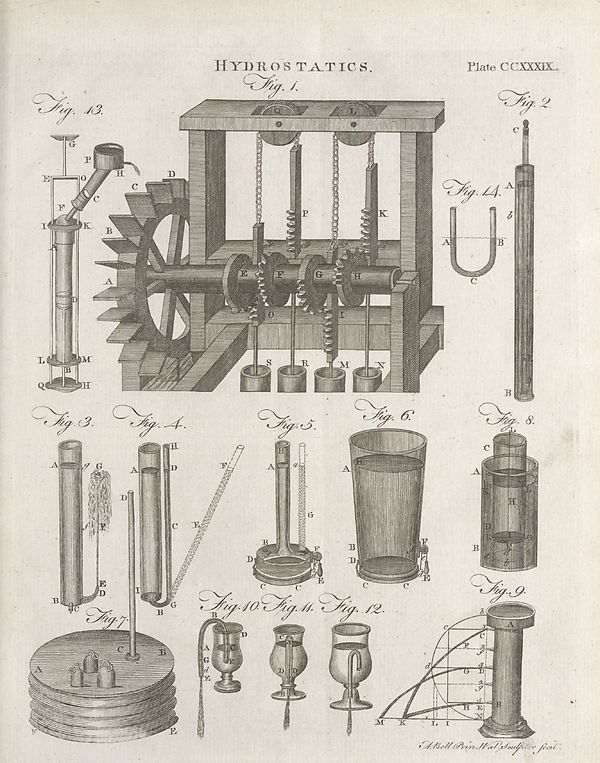
\includegraphics[width=0.85\textwidth]{../scans/page-0270-6831cc1f149b.jpg}
\caption*{Source scan: \texttt{page-0270-6831cc1f149b.jpg}}
\end{figure}

\end{document}
